%\section{State-Space Models and Bayesian Inference}
This chapter builds on the work of \cite{Doucet} and \cite{DoucetEstParamSSM} \dots \todo{cite}
% BDA3, 

Suppose we have a hidden Markov model (HMM), also called a \gls*{SSM}. Specifically, we consider a discrete-time Markov process $\{X_n; n\geq 1\}$, where each $X_n$ takes values in $\mathcal{X}$. This process is characterized by an initial distribution 
\[
X_1 \sim \mu(x_1)
\] 
and the transition density
\begin{equation}
	X_{n+1} \vert (X_n=x_n) \sim f_\theta(x_{n+1} \vert x_n) 
	\label{eq:latent_dens}
\end{equation}
for some parameter $\theta \in \Theta$. Our goal is to infer the latent states $\{X_n\}$ (or $\theta$ if it is unknown), given a sequence of noisy observations $\{Y_n; n\geq 1\}$, where each $Y_n$ takes values in the space $\mathcal{Y}$. The observation $Y_n$ is assumed to be conditionally independent of all other observations and states, given the latent state $X_n$, and is characterized by
\begin{equation}
	Y_n \vert X_n=x_n \sim g_\theta(y_n \vert x_n).
	\label{eq:obs_dens}
\end{equation}
Let $y_{1:T}=(y_1,\dots,y_T)$ denote the sequence of observations up to time $T\geq 1$. For the rest of this chapter let $\mathcal{X} \subseteq \mathbb{R}^{d_x}$, $\mathcal{Y} \subseteq \mathbb{R}^{d_y}$ and let the densities be with respect to the corresponding Lebesgue measure. 

The likelihood function $p_\theta(y_{1:n})$ is given by
\[
p_\theta(y_{1:n})=\int p_\theta(x_{1:n}, y_{1:n}) \, dx_{1:n},
\]
where $p_\theta(x_{1:n}, y_{1:n})$ is the joint density of $(X_{1:n}, Y_{1:n})$ which by Equations (\ref{eq:latent_dens})-(\ref{eq:obs_dens}) is
\[
p_\theta(x_{1:n}, y_{1:n})=\mu_\theta(x_1) \prod_{k=1}^{n} f_\theta(x_k \vert x_{k-1})\prod_{k=1}^{n} g_\theta(y_k\vert x_k).
\]
Here, the product over the transition densities \( f_\theta(x_k\vert x_{k-1}) \) captures the temporal evolution of the latent states, while the product over the likelihoods \( g_\theta(y_k \vert x_k) \) incorporates the information provided by the observations.

However, the likelihood is often intractable, necessitating Monte Carlo methods. The literature splits this setup up into two problems, filtering and smoothing. We define them as follows:
\begin{itemize}
	\item \emph{Filtering:} At each time step $n$, the goal is to sequentially approximate:
	The joint conditional distribution of the latent states given the observations,
	\[
	p_\theta(x_{1:n}\mid y_{1:n}),
	\]
	and the marginal likelihood,
	\[
	p_\theta(y_{1:n}).
	\]
	So, at time $n=1$, we approximate $p_\theta(x_1\vert y_1)$ and $p_\theta(y_1)$; at time $n=2$, we approximate $p_\theta(x_{1:2}\vert y_{1:2})$ and $p_\theta(y_{1:2})$, and so on. This sequential framework aligns directly with the setup described in the previous chapter.
	
	\item \emph{Smoothing:} The objective in smoothing is to estimate the latent states by using the entire sequence of observations $y_{1:T}$. In particular, approximating the joint conditional distribution
	\[
		p_\theta(x_{1:n}\mid y_{1:T}), \quad n=1,\dots,T,
	\]
	and the marginal conditional distributions
	\[
		p_\theta(x_n\mid y_{1:T}), \quad n=1,\dots,T.
	\]
	Because smoothing uses future observations, the resulting state estimates are generally more accurate and smoother than those obtained via filtering. This improvement is particularly beneficial when real-time estimation is not required.
\end{itemize}
That is, the difference between filtering and smoothing is whether the inference is carried out on-line (filtering) or off-line (smoothing). On-line inference is done sequentially when observations become available, and off-line inference uses a fixed number of observations. 

For the remainder of this Chapter, we suppose that $\theta$ is known. 

%%%%%% Verify this when the Chapter is done. 

\section{Filtering}
We can write the posterior density $p_\theta(x_{1:n} \vert y_{1:n})$ and the likelihood $p_\theta(y_{1:n})$ recursively for $n\geq 2$
\begin{equation*}
	%\label{eq:filt_post_lik}
	p_\theta(x_{1:n} \vert y_{1:n})=p_\theta(x_{1:n-1} \vert y_{1:n-1})\frac{f_\theta(x_n \vert x_{n-1})g_\theta(y_n \vert x_n)}{p_\theta(y_n \vert y_{1:n-1})}
\end{equation*} 
and
\begin{equation*}
	%\label{eq:filt_lik}
	p_\theta(y_{1:n})=p_\theta(y_{1:n-1}) p_\theta(y_n \vert y_{1:n-1})
\end{equation*} 
where the predictive likelihood $p_\theta(y_n \vert y_{1:n-1})$ is given by
\begin{align*}
	%\label{eq:filt_pred_lik}
	p_\theta(y_n \mid y_{1:n-1}) 
	&= \int p_\theta(y_n, x_n \mid y_{1:n-1})\,dx_n  \\
	&= \int g_\theta(y_n \mid x_n)\,p_\theta(x_n \mid y_{1:n-1})\,dx_n  \\
	&= \int g_\theta(y_n \mid x_n) f_\theta(x_n \mid x_{n-1})\,p_\theta(x_{n-1} \mid y_{1:n-1}) \,dx_{n-1:n}. 
\end{align*}
Here we are in the setup discussed in Chapter \ref{chap:MCM}, and we can for example use the \hyperref[algo:SISAR]{SISAR algorithm}. We will refer to these as particle filter algorithms. 
\begin{example}[SSM with known $\theta$]
	\label{exa:SSM_known_theta}
	Consider the following non-linear Gaussian SSM model where $\theta=(\phi, \sigma_x,\sigma_y)$ is assumed to be known. 
	\begin{align*}
		X_1 &\sim N(0,\, 1) \\
		X_t&=\phi X_{t-1}+\sin(X_{t-1})+\sigma_x V_t, \quad V_t \sim N(0, \, 1) \\
		Y_t&=X_t+\sigma_y W_t, \quad W_t \sim N(0, \, 1).
	\end{align*}
	We set $\phi=0.7$, $\sigma_x=1$, $\sigma_y=1$, with a time horizon of $T=50$, and $N=1000$ particles. 
	A single simulation of the SSM is visualized in Figure~\ref{fig:hidden_obs_known_theta}.
	
	Our goal is to compare the performance of SIS, SISR, and SISAR for estimating the latent state $X_t$. Performance is evaluated using the root mean squared error (RMSE), with the estimates obtained from 10,000 Monte Carlo replications. For SISR and SISAR we use stratified sampling during the resampling step. The R code for this simulation is available at \url{https://github.com/BjarkeHautop/master-thesis/tree/main/R}.
	
	\begin{figure}
		\centering
		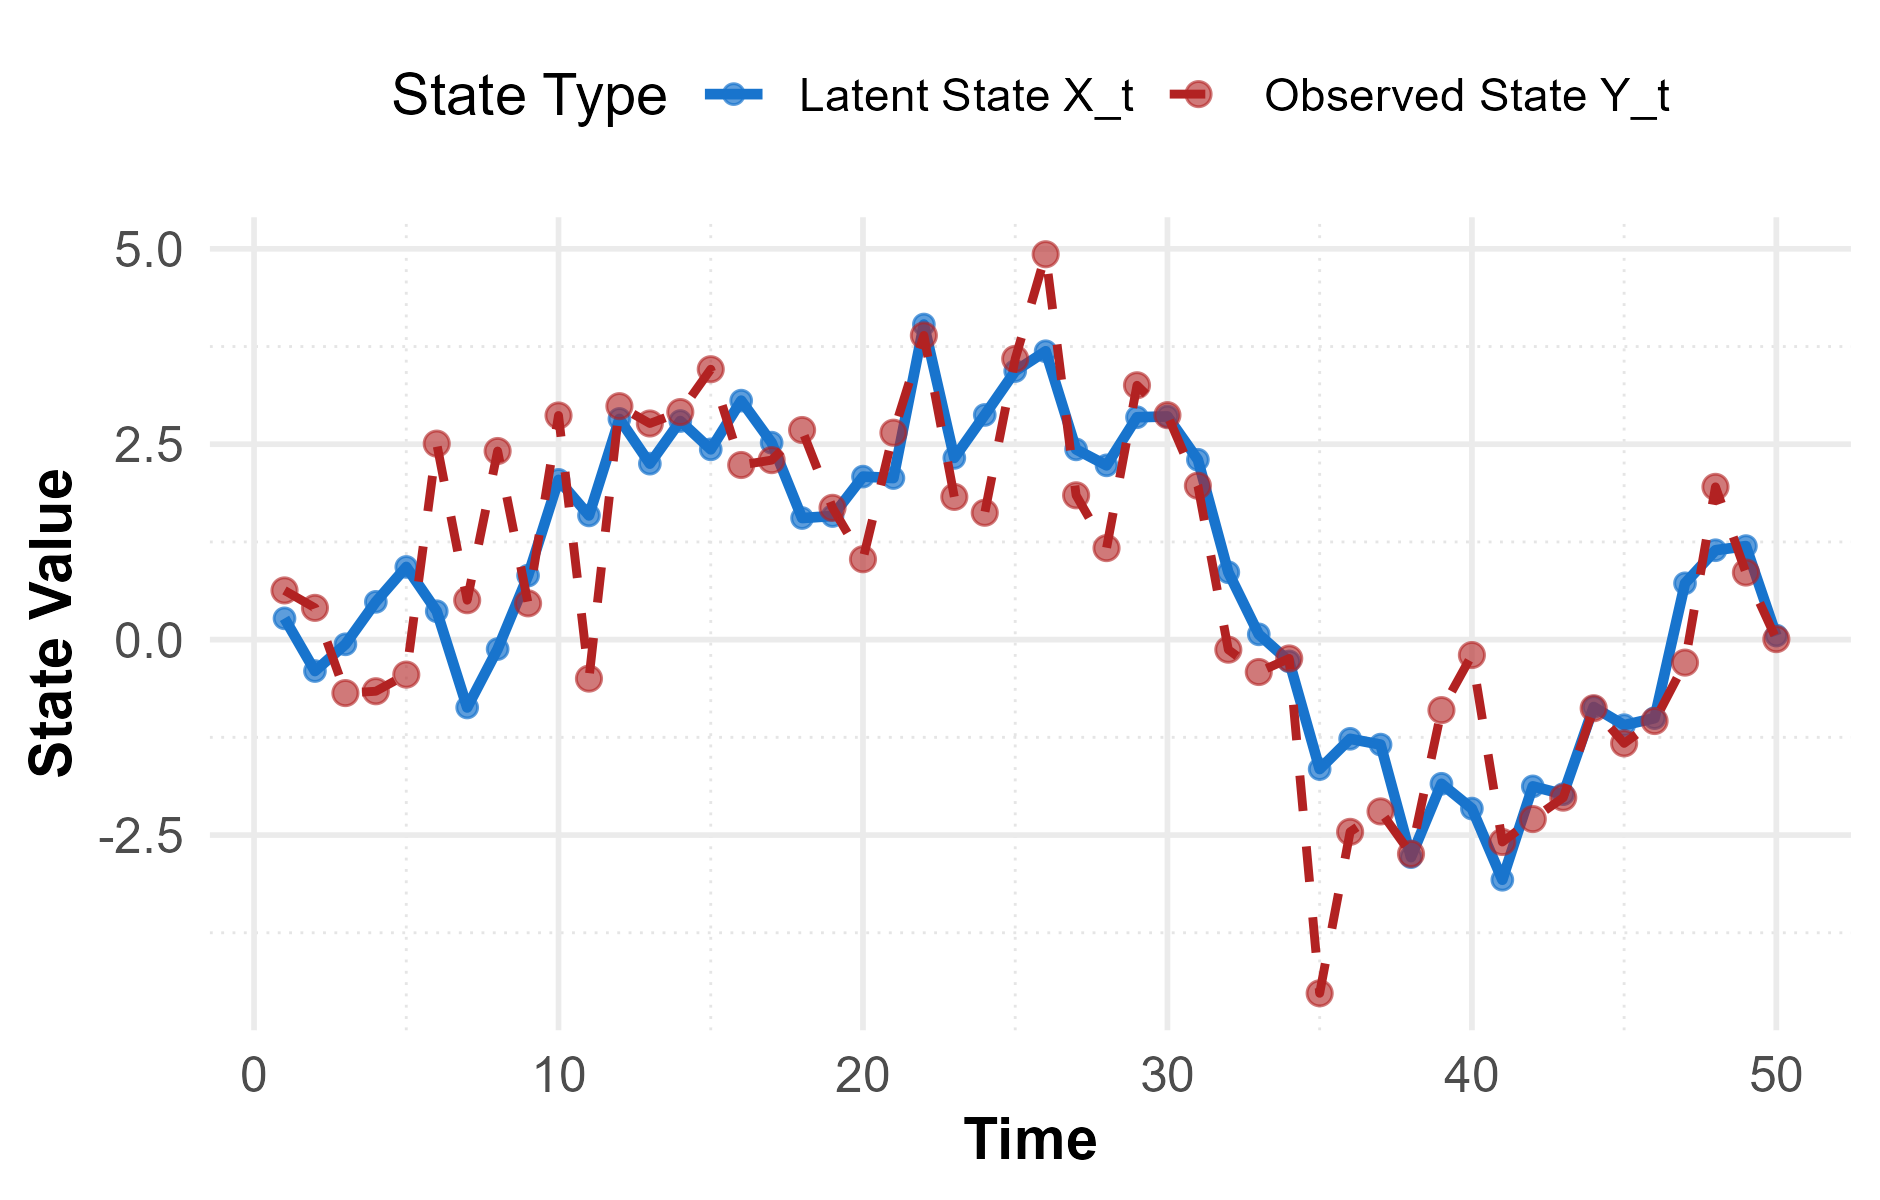
\includegraphics{Latent_obs_example3.1.png}
		\caption{A simulated trajectory of the \gls*{DGP} in Example~\ref{exa:SSM_known_theta}}
		\label{fig:hidden_obs_known_theta}
		% Convert to pdf see https://www.overleaf.com/learn/latex/Inserting_Images Generating high-res and low-res images
	\end{figure}	
	The results are visualized in Figure~\ref{fig:particle_filter_estimates} and in Table~\ref{tab:performance}, expressed as mean (standard deviation). We see that SIS performs the worst, while SISR and SISAR almost gives the same estimates. However, SISAR is computationally more efficient since it does not resample at every time step. The poorer performance of SIS is due to weight degeneracy, where almost all the weight is carried by a few particles.
	
	\begin{figure}
		\centering
		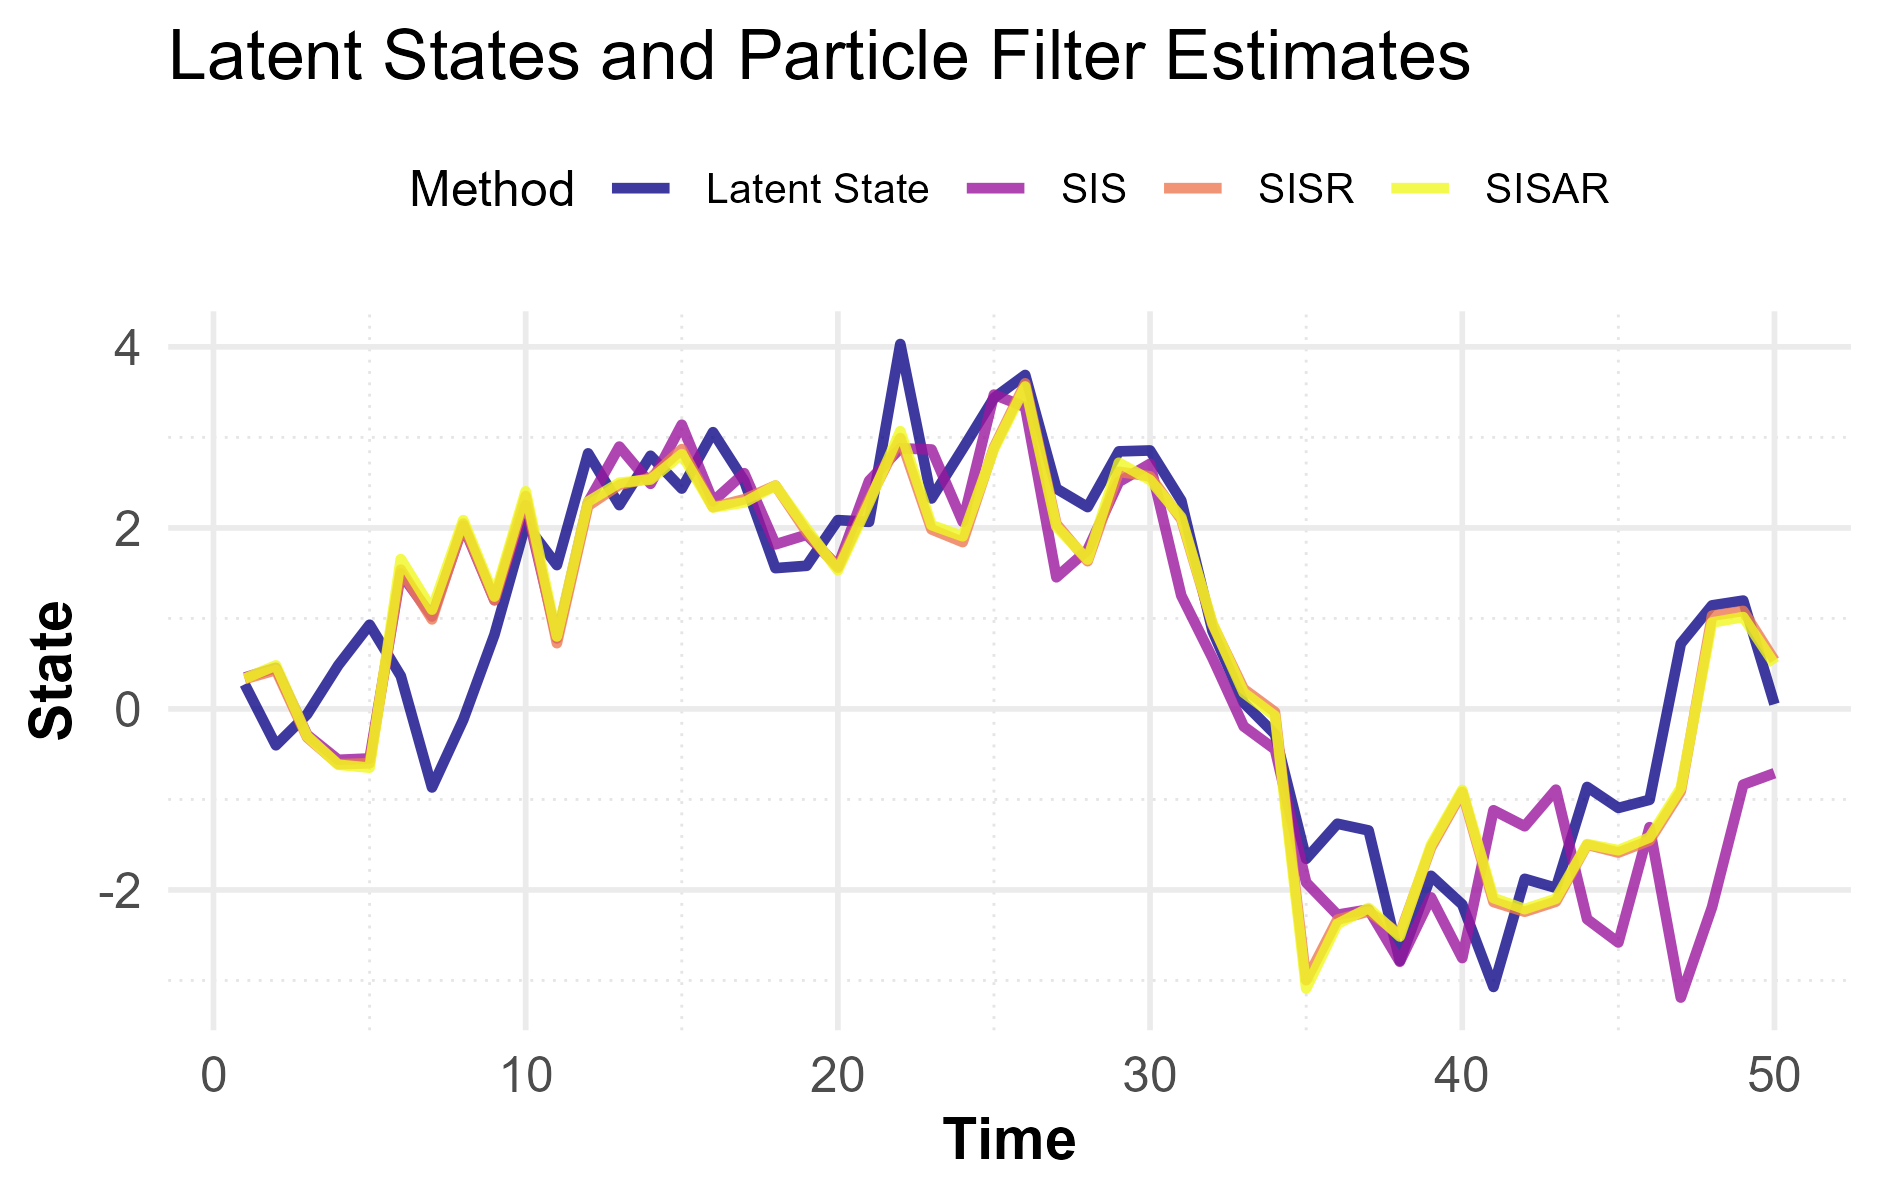
\includegraphics{example_3.1_estimates.png}
		\caption{The particle filter estimates of the latent state of the \gls*{DGP} in Example~\ref{exa:SSM_known_theta}. Note, that SISR and SISAR almost produces the same estimates.}
		\label{fig:particle_filter_estimates}
		% Convert to pdf see https://www.overleaf.com/learn/latex/Inserting_Images Generating high-res and low-res images
	\end{figure}	
	
	\begin{table}
		\centering
		\begin{tabular}{lccc}
			\toprule
			Algorithm & SIS & SISR & SISAR \\
			\midrule
			RMSE      & 1.08 (0.18) & 0.75 (0.09) & 0.75 (0.09) \\
			\bottomrule
		\end{tabular}
		\caption{Comparison of RMSE performance for SIS, SISR, and SISAR algorithms based on 10,000 Monte Carlo replications for Example~\ref{exa:SSM_known_theta}. The values are the estimated means (standard deviations).}
		\label{tab:performance}
	\end{table}
\end{example}

\section{Smoothing}
\subsection{Forward-Backward Recursions}
By doing a decomposition of the joint distribution $p_\theta(x_{1:T} \vert y_{1:T})$ we see that conditional on $y_{1:T}$ that $\{X_n\}$ is an non-homogeneous Markov process
\begin{align}
	p_\theta(x_{1:T} \vert y_{1:T})&=p_\theta(x_{1:T} \vert  y_{1:T})\prod_{n=1}^{T-1}p_\theta(x_n \vert x_{n+1}, y_{1:T}) \nonumber \\
	&=p_\theta(x_T \vert y_{1:T})\prod_{n=1}^{T-1}p_\theta(x_n \vert x_{n+1}, y_{1:n}), \label{eq:forward-backward}  
\end{align}
where we in the 2nd equality used the Markov property. Using Bayes' Theorem, we can write the marginal $p_\theta(x_n \vert x_{n+1}, y_{1:n})$ as
\begin{equation}
	p_\theta(x_n \vert x_{n+1}, y_{1:n}) = \frac{f_\theta(x_{n+1} \vert x_n) p_\theta(x_n \vert y_{1:n})}{p_\theta(x_{n+1} \vert y_{1:n})}.
	\label{eq:marginal_FBR}
\end{equation}
By integrating out $(x_{1:n-1}, x_{n+1:T})$ in  \cref{eq:forward-backward} we have that the marginal distribution $p_\theta(x_n \vert y_{1:T})$ is given by
\begin{align}
	p_\theta(x_n \vert y_{1:T})&=\int p_\theta(x_{1:T} \vert y_{1:T})\, dx_{1:n-1} \, dx_{n+1:T} \nonumber \\
	&=\int p_\theta(x_T \vert y_{1:T})\prod_{k=1}^{T-1}p_\theta(x_k \vert x_{k+1}, y_{1:k}) \, dx_{1:n-1} \, dx_{n+1:T} \nonumber \\
	&=\int p_\theta(x_T \vert y_{1:T})\prod_{k=1}^{T-1}\frac{f(x_{k+1} \vert x_k) p_\theta(x_k \vert y_{1:k})}{p_\theta(x_{k+1} \vert y_{1:k})} \, dx_{1:n-1} \, dx_{n+1:T} \nonumber \\
	&=p_\theta(x_n \vert y_{1:n}) \int \frac{f(x_{n+1} \vert x_n)}{p_\theta(x_{n+1} \vert y_{1:n})}p_\theta(x_{n+1} \vert y_{1:T}) \, dx_{n+1}. \label{eq:marginal_backwards}
\end{align}
This is referred to as forward-backward smoothing, as a forward pass yields $\{p_\theta(x_n \vert y_{1:n})\}_{n=1}^{T}$, which can then be used in a backward pass to obtain $\{p_\theta(x_n \vert y_{1:T})\}_{n=1}^T$.

\subsection{Forward-Filtering Backward-Sampling (FFBSm)}
A common method for drawing samples from the joint smoothing distribution \(p_\theta(x_{1:T} \vert y_{1:T})\) is the Forward-Filtering Backward-Sampling with marginalization (FFBSm) method. This method proceeds in two steps:

\begin{enumerate}
	\item \textbf{Forward filtering:} The filtering distributions \(\{p_\theta(x_n \vert y_{1:n})\}_{n=1}^{T}\) are approximated using a filtering method, such as those described in Chapter~\ref{chap:MCM}. In this step, particles are used to approximate the filtering distributions, with each particle \(x_n^{(j)}\) associated with a weight \(W_n^{(j)}\), where \(W_n^{(j)}\) is the normalized weight of the particle \(x_n^{(j)}\). The weight reflects how well the particle approximates the target distribution \(p_\theta(x_n \mid y_{1:n})\). These weights are essential for guiding the importance of each particle in subsequent sampling steps.
	
	\item \textbf{Backward sampling:} 
	\begin{itemize}
		\item First, we sample the final state \( X_T \) from the distribution \( p_\theta(x_T \mid y_{1:T}) \), which is proportional to the forward-filtered particles at time \(T\). Since the forward filter gives a weighted sample \( \{ x_T^{(j)} \} \) we sample $X_T^{(i)}$ with probability \( W_T^{(j)} \). 
		
		\item For each time step \( n=T-1,T-2,\dots,1 \), we sample the state \( X_n \) given the sampled state \( X_{n+1} \) and the observations \( y_{1:n} \). The sampling procedure is based on the backward conditional distribution \( p_\theta(x_n \mid X_{n+1}, y_{1:n}) \), which is proportional to the joint likelihood of the transition from \( x_n \) to \( x_{n+1} \) and the forward filtering distribution. More formally, we have:
		\[
		p_\theta(x_n \mid X_{n+1}, y_{1:n}) = \frac{ f_\theta(X_{n+1} \mid x_n) p_\theta(x_n \mid y_{1:n}) }{ p_\theta(X_{n+1} \mid y_{1:n}) },
		\]
		where \( f_\theta(X_{n+1} \mid x_n) \) is the state transition density, and \( p_\theta(x_n \mid y_{1:n}) \) is the forward filtering distribution for state \( x_n \). To sample \( X_n^{(i)} \), we first compute the backward weights \( \tilde{w}_n^{(j)} \), which adjust the forward weights by the transition probability:
		\[
		\tilde{w}_n^{(j)} = W_n^{(j)} f_\theta(X_{n+1}^{(j)} \mid x_n^{(j)}).
		\]
		
		\item Finally, we normalize the backward weights:
		\[
		\tilde{W}_n^{(j)} = \frac{\tilde{w}_n^{(j)}}{\sum_{j=1}^N \tilde{w}_n^{(j)}}.
		\]
		Then, we sample an index \( k \) from \( \{1, 2, \dots, N\} \) with probability \( \tilde{W}_n^{(k)} \), and set \( X_n^{(i)} = x_n^{(k)} \). This step ensures that the sampled trajectory is consistent with the joint smoothing distribution \( p_\theta(x_{1:T} \mid y_{1:T}) \).
	\end{itemize}
\end{enumerate}
In summary, the forward weights \(W_n^{(j)}\) capture the likelihood of each particle given the observations up to time \(n\), while the backward weights \(\tilde{w}_n^{(j)}\) adjust for the transition probabilities between states. 
The pseudocode for the FFBSm algorithm is provided in Algorithm \ref{algo:FFBSm}. The time complexity of the FFBSm algorithm is \(O(N^2T)\). This time complexity arises the backward sampling step, which involves three nested loops. Hence, the total time complexity is \(O(N^2T))\). This is significantly slower than the algorithms in the previous chapter that had a complexity of \(O(NT)\).
\begin{algorithm}[H]
	\caption{Forward-Filtering Backward-Sampling (FFBSm)}
	\label{algo:FFBSm}
	\begin{algorithmic}[1]
		\State \textbf{Input:} Observations \(y_{1:T}\), number of particles \(N\), initial distribution \(\mu(x_1)\), state transition density \(f_\theta(x_{n+1}\mid x_n)\), observation density \(g_\theta(y_n\mid x_n)\)
		\State \textbf{Forward Filtering:} 
		\State Use a forward filtering algorithm (described in Chapter~\ref{chap:MCM}) to obtain, for each \(n=1,\dots,T\), the particle approximation \(\{x_n^{(j)}, W_n^{(j)}\}_{j=1}^N\) of \(p_\theta(x_n\mid y_{1:n})\), where \( W_n^{(j)} \) are the normalized weights
		\For{\(i=1,\dots,N\)}
		\State \textbf{Backward Sampling:}
		\State Sample index \(k\) from \(\{1,\dots,N\}\) with probability \(W_T^{(k)}\)
		\State Set \(X_T^{(i)} = x_T^{(k)}\)
		\For{\(n=T-1, T-2, \dots, 1\)}
		\For{\(j=1,\dots,N\)}
		\State Compute backward weights:
		\[
		\tilde{w}_n^{(j)} = W_n^{(j)}\, f_\theta\Bigl(X_{n+1}^{(i)}\mid x_n^{(j)}\Bigr)
		\]
		\EndFor
		\State Normalize: \( \tilde{W}_n^{(j)} \leftarrow \frac{\tilde{w}_n^{(j)}}{\sum_{j=1}^N \tilde{w}_n^{(j)}} \)
		\State Sample index \(k\) from \(\{1,\dots,N\}\) with probability \(\tilde{W}_n^{(k)}\)
		\State Set \(X_n^{(i)} = x_n^{(k)}\)
		\EndFor
		\EndFor
		\State \textbf{Output:} \(N\) sampled trajectories \(\{X_{1:T}^{(i)}\}_{i=1}^N\)
	\end{algorithmic}
	% MAKE ALGORITHM MORE LIKE PMMH? I.E. EXPLICIT INPUT OUTPUT
\end{algorithm}

Another approach for smoothing is the Generalised Two-Filter Formula, as discussed in \cite{BRESLER01021986}.

\begin{example}[Example~\ref{exa:SSM_known_theta} continued]
	\label{exa:SSM_known_theta_cont}
	We continue Example~\ref{exa:SSM_known_theta} with the same model and setup, now performing smoothing using the \hyperref[algo:FFBSm]{FFBSm} algorithm. The forward pass is carried out using the \hyperref[algo:SISAR]{SISAR} algorithm with stratified resampling. Due to the computational cost of this approach, particularly the $O(N^2T)$ backward sampling step, the implementation was done in Julia for efficiency. The Julia code is available at \url{https://github.com/BjarkeHautop/master-thesis/tree/main/Julia}. 
	
	An example trajectory of the latent state $X_t$ and the filtering estimate from the SISAR algorithm alongside the smoothed estimate of the FFBSm algorithm is shown in Figure~\ref{fig:filt_smooth_est}.   
	\begin{figure}
		\centering
		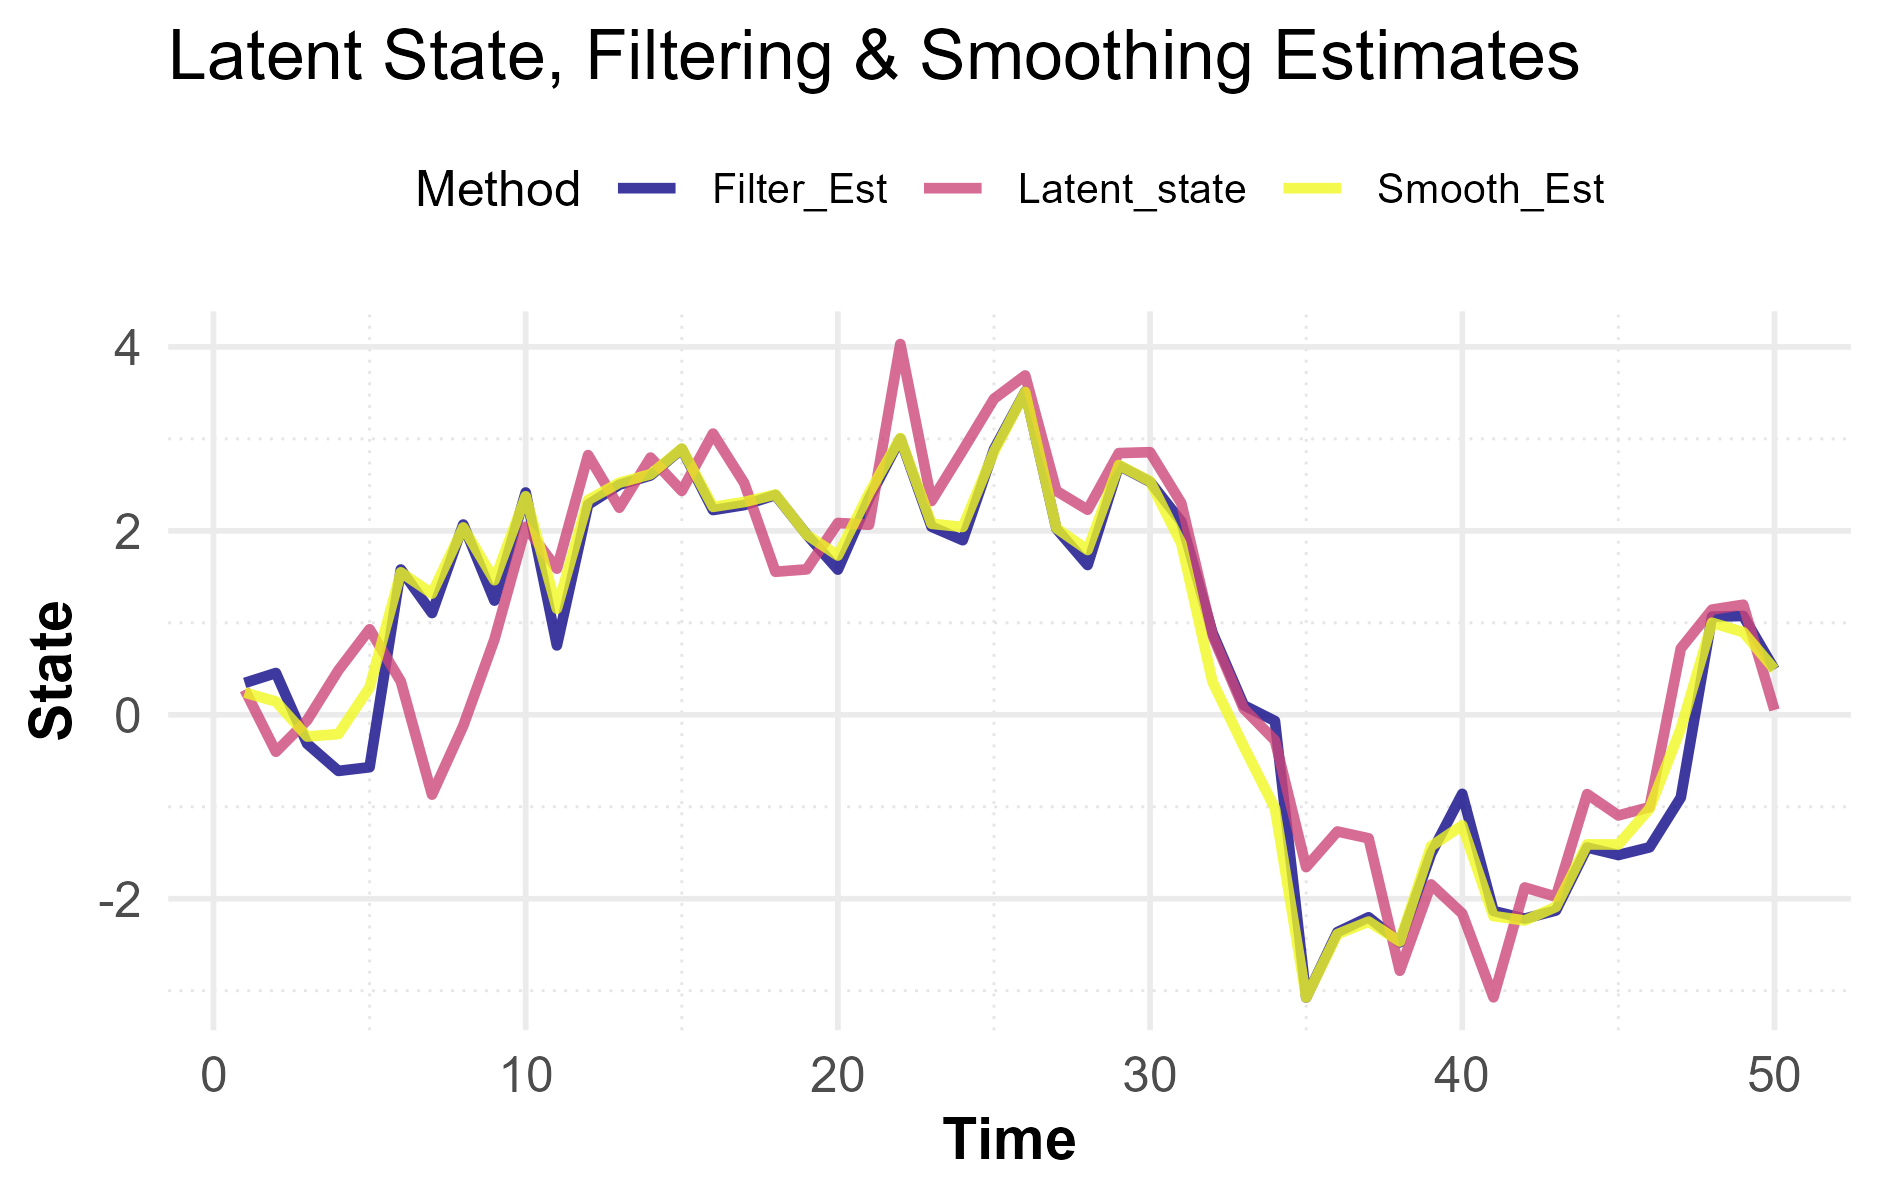
\includegraphics{Example_3.3_estimates.png}
		\caption{A simulated trajectory of the SSM in  Example~\ref{exa:SSM_known_theta_cont} alongside the filtering and smoothing estimates.}
		\label{fig:filt_smooth_est}
		% Convert to pdf see https://www.overleaf.com/learn/latex/Inserting_Images Generating high-res and low-res images
	\end{figure}
	We estimate the RMSE and standard deviation based on 10,000 Monte Carlo iterations.  Table~\ref{tab:performance_ext} summarizes the results, including values from filtering algorithms for comparison.
	\begin{table}
		\centering
		\begin{tabular}{lcccc}
			\toprule
			Algorithm & SIS & SISR & SISAR & FFBSm \\
			\midrule
			RMSE      & 1.08 (0.18) & 0.75 (0.09) & 0.75 (0.09) & 0.69 (0.08) \\
			\bottomrule
		\end{tabular}
		\caption{Comparison of RMSE performance for SIS, SISR, SISAR, and FFBSm algorithms based on 10,000 Monte Carlo replications for Example~\ref{exa:SSM_known_theta_cont}. The values are the estimated means (standard deviations).}
		\label{tab:performance_ext}
	\end{table}
\end{example}


